\textit{Burp Suite}\cite{burp} (figura \ref{fig:burp-logo}) es una de las herramientas preferidas para muchos profesionales de seguridad, pentesters, bug hunters, etc.  Es una plataforma integrada para realizar evaluaciones de seguridad a aplicaciones web. Esta diseñada para apoyar la metodología de una evaluación manual, y proporciona un completo control sobre las acciones a realizar, además de un análisis profundo de los resultados. \textit{Burp Suite} contiene varias herramientas que trabajan juntas para realizar virtualmente cualquier tarea que pueda ser encontrada en las evaluaciones. Puede automatizar todo tipo de tareas de manera personalizada, y permite combinar técnicas manuales y automáticas para hacer las pruebas más rápidas, más confiables y mas divertidas.

\begin{figure}[h]
    \centering
    
\includegraphics[width=0.30\textwidth]{images/sections/tools/burp.png}
    \caption{Logo de \textit{Burp Suite}}
    \label{fig:burp-logo}
\end{figure}

Los componentes claves de \textit{Burp} son:
\begin{itemize}
    \item Un \textbf{Proxy} de interceptación, el cual permite inspeccionar y modificar el tráfico entre el navegador y la aplicación objetivo.
    \item Un \textbf{Spider} de conocimiento de la aplicación, para recorrer contenidos y funcionalidades.
    \item Un escáner (\textbf{Scanner}) avanzado para la aplicación web, para automatizar la detección de varios tipos de vulnerabilidades.
    \item Una herramienta de repetición, \textbf{Repeater}, para manipular y reenviar solicitudes individuales.
    \item Una herramienta de secuencia (\textbf{Sequencer}), para evaluar la aleatoriedad de los tokens de sesión.
    \item Es ampliable, permite escribir fácilmente plugins propios, para realizar tareas altamente personalizadas y complejas dentro de \textit{Burp Suite}.
\end{itemize}

Entre las características principales se encuentran:
\begin{itemize}
    \item Permite realizar de forma automatizada pruebas de exploración y escaneo de vulnerabilidades.
    \item Contiene un escáner de vulnerabilidades avanzado para pruebas manuales.
    \item Lógica de exploración de vanguardia.
    \item Presentación clara y detallada de vulnerabilidades, con recomendaciones y los payloads utilizados.
    \item Interceptar el tráfico del navegador mediante el Proxy (man-in-the-middle).
    \item Ataques automatizados y personalizados usando \textit{Burp Intruder}.
    \item Contiene herramientas de prueba manuales avanzadas.
    \item Brinda diferentes métodos y técnicas de conexión a las aplicaciones Web.
\end{itemize}

A continuación, en la figura \ref{fig:burp-example}, se muestra la herramienta de \textit{Proxy} capturando la red, y mostrando el contenido de una \textit{request} a \textit{GitHub}.

\begin{figure}[h]
    \centering
    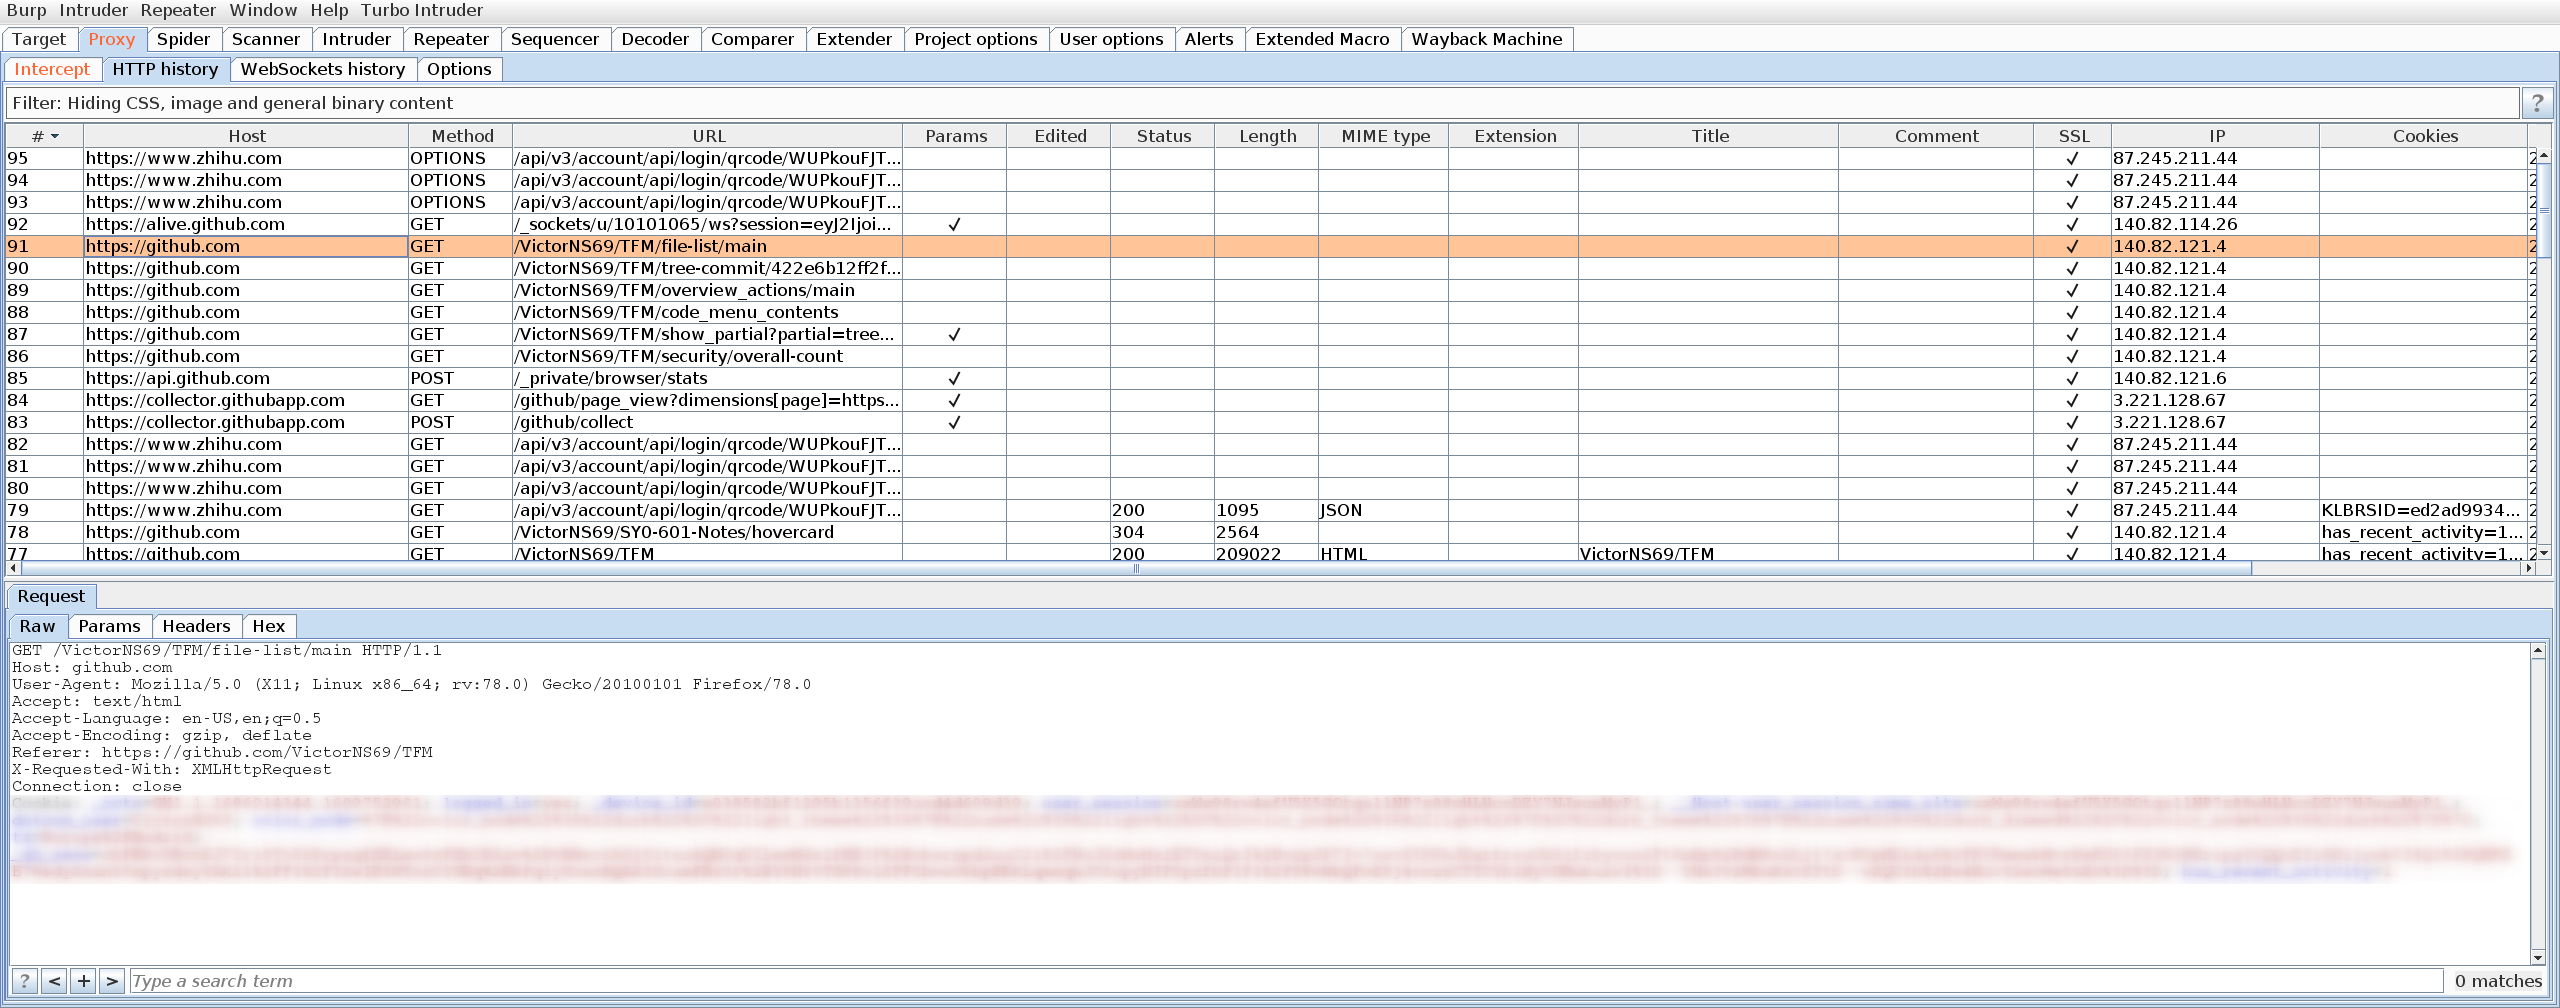
\includegraphics[width=1.0\textwidth]{images/sections/tools/captura-burp.png}
    \caption{Ejemplo de uso de \textit{Burp Suite}}
    \label{fig:burp-example}
\end{figure}